\chapter{Tactics}
\label{chapter:tactics}
\begin{quotation}
\textit{Probability theory can tell us how our hypothesis fares relative to the alternatives that we have specified; it does not have the creative imagination to invent new hypotheses for us.}
\begin{flushright}E.T. \cite{Jaynes}\end{flushright}
\end{quotation}

%%% Beyond the age of information is the age of choices.
%%% -- Charles Eames

%%% Correlation doesn't imply causation, but it does waggle its eyebrows suggestively and gesture furtively while mouthing 'look over there'.
%%% -- Randall Munroe

%%% \textit{We learn about who someone is by the choices they make when the choice isn't obvious.}
%%% \begin{flushright}Ben Casnocha\end{flushright}


%%% "Very recently - in just the last few decades - the human species has acquired a great deal of new knowledge about human rationality. The most salient example would be the heuristics and biases program in experimental psychology. There is also the Bayesian systematization of probability theory and statistics; evolutionary psychology; social psychology. Experimental investigations of empirical human psychology; and theoretical probability theory to interpret what our experiments tell us; and evolutionary theory to explain the conclusions. These fields give us new focusing lenses through which to view the landscape of our own minds. With their aid, we may be able to see more clearly the muscles of our brains, the fingers of thought as they move. We have a shared vocabulary in which to describe problems and solutions. Humanity may finally be ready to synthesize the martial art of mind: to refine, share, systematize, and pass on techniques of personal rationality."
%%% -- Eliezer Yudkowsky

%%% Your calendar never lies. All we have is our time. The way we spend our time is our priorities, is our "strategy." Your calendar knows what you really care about. Do you?
%%% -- Tom Peters, HT Ben Casnocha

%%% When things are hard to understand, people who suspect they're nonsense generally keep quiet.
%%% -- Paul Graham

%%% "Don't worry about what anybody else is going to do.do The best way to predict the future is to invent it."
%%% - Alan Kay

%%% "The imagination of nature is far, far greater than the imagination of man."
%%% - Richard Feynman

%%% “SUCCESS: to laugh often and much; to win the respect of intelligent people and the affection of children; to earn the appreciation of honest critics and endure the betrayal of false friends; to appreciate beauty, to find the best in others; to leave the world a bit better, whether by a healthy child, a garden patch or a redeemed social condition ; to know even one life has breathed easier because you have lived. This is to have succeeded.” Emerson

\lettrine{W}{e} present a Bayesian model for tactical decision-making in real-time strategy games. The main idea is to adapt the model to inputs from (possibly) biased heuristics. We evaluated the model in prediction of the enemy tactics on professional gamers data. This work was accepted for publication at Computational Intelligence in Games (CIG) 2012 in Grenada \citep{SYNNAEVE:Tactics} and will be presented at the Computer Games Workshop of the European Conference of Artificial Intelligence (ECAI) 2012 \citep{SYNNAEVE:TacticsECAI}.

\ifthenelse{\equal{\myebookformat}{false}}{
\chaptertoc
}{}

\begin{itemize}
\item Problem: make the most efficient tactical decisions (attacks and defenses) in the absolute (knowing everything: armies positions, players intentions, effects of each possible actions).
\item Problem that we solve: make the most efficient tactical decisions (in average) knowing what we saw from the opponent and our model of the game. 
\item Type: prediction is problem of \textit{inference} or \textit{plan recognition} from \textit{partial observations}; adaptation given what we know is a problem of \textit{decision-making under uncertainty}. 
\item Complexity: the complexity of tactical moves has not been studied particularly, as ``tactics'' are hard to bound. If taken form the low-level actions that units perform to produce tactics, the complexity is that of micro-management performed on the whole map and is detailed in section~\ref{sec:rtsaichallenges}. Players and AI build abstractions on top of that, which enables them to reason about enemy tactics and infer what they should do from only partial observations. For these reasons, we think that tactics, at this abstract level, can be modeled as a \glos{pomdp} with partial observations of the opponent's tactics (identifying them from low-level observations is already an arduous task), actions as our tactics, and transition probabilities defined by player's skills and the game state. %at least \textsc{pspace}-complete\footnote{the space of tactics can be seen as a finite combination of possible military actions and geographical positions, and thus tactics can be modeled as a \glos{pomdp}}. %EXPTIME-complete as for Chess and Go \citep{Robson83}). 
Our solutions are real-time on a laptop.
\end{itemize}

\begin{figure}[!ht]
\begin{center}
\includegraphics[width=13cm]{images/starcraft_bbq_concept_TACTICS.pdf}
\end{center}
\label{fig:conceptTACTICS}
\caption{Information-centric view of the architecture of the bot, the part concerning this chapter (tactics) is in the dotted rectangle. Dotted arrows represent constraints on what is possible, plain simple arrows represent simple (real) values, either from data or decisions, and double arrows represent probability distributions on possible values. The grayed surfaces are the components actuators (passing orders to the game).}
\end{figure}
%%% \begin{itemize}
%%% \item Problem: choose which tactical actions/goals to persue, peform the action
%%% \item Complexity: incompleteness/uncertainty problem, lot of low level information to handle, w.r.t. full and higher level information, simple.
%%% \item State of the art: \citep{SORTS, Weber2010cr, UCT, CadenaG11}
%%% \item Our take: low level heuristics that we learn to adapt to
%%% \item Results: 
%%% \item Conclusion and perspectives: still enabled for meta-game, and even in-game, adaptation. Could learn the action sequences of tactics from replays ($\approx$HMM).
%%% \end{itemize}

\section{What are Tactics?}
\subsection{A Tactical Abstraction}
In their study on human like characteristics in RTS games, Hagelb\"{a}ck and Johansson \cite{HagelbackCIG10} found out that ``tactics was one of the most successful indicators of whether the player was human or not''. Tactics are in between strategy (high-level) and micro-management (lower-level), as seen in Fig.~\ref{fig:sc_abstraction_times}. When players talk about specific tactics, they use a specific vocabulary which represents a set of actions and compresses subgoals of a tactical goal in a sentence. %(see Fig.~\ref{fig:conceptTACTICS}). 

Units have different abilities, which leads to different possible tactics. Each faction has invisible (temporarily or permanently) units, flying transport units, flying attack units and ground units. Some units can only attack ground or air units, some others have splash damage attacks, immobilizing or illusion abilities. Fast and mobile units are not cost-effective in head-to-head fights against slower bulky units. We used the gamers' vocabulary to qualify different types of tactics: 
\begin{itemize}
    \item \textit{ground} attacks (raids or pushes) are the most normal kind of attacks, carried by basic units which cannot fly,
    \item \textit{air} attacks (air raids), which use flying units' mobility to quickly deal damage to undefended spots.
    \item \textit{invisible} attacks exploit the weaknesses (being them positional or technological) in detectors of the enemy to deal damage without retaliation,
    \item \textit{drops} are attacks using ground units transported by air, combining flying units' mobility with cost-effectiveness of ground units, at the expense of vulnerability during transit.
\end{itemize}
This will be the only four types of tactics that we will use in this chapter: \textit{how} did the player attack or defend? That does not mean that it is an exhaustive classification, nor that our model can not be adapted a) to other types of tactics b) to dynamically learning types of tactics.

RTS games maps, StarCraft included, consist in a closed arena in which units can evolve. It is filled with terrain features like uncrossable terrain for ground units (water, space), cliffs, ramps, walls. Particularly, each RTS game which allows production also give some economical (gathering) mechanism and so there are some resources scattered on the map, where players need to go collect. It is way more efficient to build expansion (auxiliary bases) to collect resources directly on site. So when a player decides to attack, she has to decide \textit{where} to attack, and this decision takes into account \textit{how} it can attack different places, due to their geographical remoteness, topological access posibilities and defense strengh. Choosing \textit{where} to attack is a complex decision to make: of course it is always wanted to attack poorly defended economic expansions of the opponent, but the player has to consider if it places its own bases in jeopardy, or if it may trap her own army. With a perfect estimator of battles outcomes (which is a hard problem due to terrain, army composition combinatorics and units control complexity), and perfect information, this would result in a game tree problem which could be solved my $\alpha-\beta$. Unfortunately, StarCraft is a partial observation game with complex terrain and fight mechanics.

\subsection{Our Approach}
The idea is to have (most probably biased) lower-level heuristics from units observations which produce information exploitable at the tactical level, and take advantage of strategic inference too. 
For that, we propose a model which can either predict enemy attacks or give us a distribution on \textit{where} and \textit{how} we should attack the opponent. Information from the higher-level strategy \citep{SYNNAEVE:StratPred,SYNNAEVE:OpeningPred} (Chapter~\ref{chapter:strategy}) constrains what types of attacks are possible. As shown in Fig.~\ref{fig:conceptTACTICS}, information from units' positions (or possibly an enemy units particle filter as in \citep{weber2011aiide} or Chapter~\ref{chapter:perspectives}) constrains where the armies can possibly be in the future. In the context of our StarCraft bot, once we have a decision: we generate a goal (attack order) passed to units groups, which set the objectives of the low-level Bayesian units control model \citep{SYNNAEVE:Micro} (Chapter~\ref{chapter:micro}).


\section{Related Work}

On spatial reasoning, \cite{Pottinger00} described the \textit{BANG} engine implemented for the game Age of Empires II (Ensemble Studios), which provides terrain analysis functionalities to the game using influence maps and areas with connectivity information. 
\cite{Forbus2002} presented a tactical qualitative description of terrain for wargames through geometric and pathfinding analysis. \cite{Hale08} presented a 2D geometric navigation mesh generation method from expanding convex regions from seeds. \cite{Perkins2010} automatically extracted choke points and regions of StarCraft maps from a pruned Voronoi diagram, which we used for our regions representations. 

\cite{Hladky_anevaluation} benchmarked hidden semi-Markov models (HSMM) and particle filters in first person shooter games (FPS) units tracking. They showed that the accuracy of occupancy maps was improved using movement models (learned from the player behavior) in HSMM. \cite{particlefiltergameAI} used a particle filter for player position prediction in a FPS. \cite{Kabanza2010} improve the probabilistic hostile agent task tracker (PHATT \citep{PHATT}, a simulated HMM for plan recognition) by encoding strategies as HTN, used for plan and intent recognition to find tactical opportunities. \cite{weber2011aiide} used a particle model for hidden units' positions estimation in StaCraft.

\cite{LTW} used case-based reasoning (CBR) to perform dynamic tactical plan retrieval (matching) extracted from domain knowledge in Wargus. \cite{Ontanon2007} based their real-time case-based planning (CBP) system on a plan dependency graph which is learned from human demonstration in Wargus. A case based behavior generator spawn goals which are missing from the current state and plan according to the recognized state. In \citep{Mishra2008,metalevelbehavioradaptrts}, they used a knowledge-based approach to perform situation assessment to use the right plan, performing runtime adaptation by monitoring its performance. \cite{CBR-RL} combined CBR and reinforcement learning to enable reuse of tactical plan components. 
\cite{Bakkes09} used richly parametrized CBR for strategic and tactical AI in Spring (Total Annihilation open source clone). 
\cite{CadenaG11} used fuzzy CBR (fuzzy case matching) for strategic and tactical planning (including expert knowledge) in StarCraft. \cite{Chung05} applied Monte-Carlo planning for strategic and tactical planning to a capture-the-flag mod of Open RTS. \cite{UCT} applied upper confidence bounds on trees (UCT: a MCTS algorithm) to tactical assault planning in Wargus. 

In Starcraft, \cite{Weber2010cr,WeberCIG10} produced tactical goals through reactive planning and goal-driven autonomy, finding the more relevant goal(s) to follow in unforeseen situations. 
\cite{SORTS} used a cognitive approach mimicking human attention for tactics and units control in ORTS. \cite{PonsenMSA06} developed an evolutionary state-based tactics generator for Wargus. %On influence maps, \cite{teamCompositionRTS} studied team composition and maneuvering by learning a self-organizing map, while \cite{HagelbackJ08} presented a multi-agent potential field based bot .....
Finally, Avery et al. \cite{Avery09} and Smith et al. \cite{SmithCIG10} co-evolved influence map trees for spatial (tactical) reasoning in RTS games. 

\section{Perception and Tactical Goals}
\subsection{Space Representation}
The \textit{maps} on which we play restrain movement and vision of ground units (flying units are not affected). As ground units are much more prevalent and more cost-efficient than flying units, being able to reason about terrain particularities is key for tactical reasoning. For that, we clustered the map in regions. 
\newacronym{BWTA}{BWTA}{BroodWar Terrain Analyser}
We used two kinds of regions: 
\begin{itemize}
    \item \glos{BWTA}\footnote{http://code.google.com/p/bwta/} regions and choke-dependent (choke-centered) regions (CDR). BWTA regions are obtained from a pruned Voronoi diagram on walkable terrain \citep{Perkins2010} and give regions for which chokes are the boundaries. We will note this regions ``Reg'' or regions.
    \item As battles often happens at chokes, choke-dependent regions are created by doing an additional (distance limited) Voronoi tesselation spawned at chokes, its regions set is $(regions \setminus chokes) \cup chokes$. We will note this regions ``CDR'' or choke-dependent regions.
\end{itemize}
Figure~\ref{fig:terrainanalysis} illustrate regions and choke-dependent regions (CDR). Results for choke-dependent regions are not fully detailed. Figure~\ref{fig:BWTA} shows a real StarCraft map and its decomposition into regions with BWTA.

\begin{figure}[!h]
\begin{center}
\includegraphics[width=16cm]{images/terrain_analysis.png}
\caption{A very simple map on the left, which is transformed into regions (between chokes in dotted red lines) by Voronoi tessellation and clustering. These plain regions (numbers in red) are then augmented with choke-dependent regions (letters in blue)}%: $CDR = (regions \setminus chokes)) \cup chokes$.}
\label{fig:terrainanalysis}
\end{center}
\end{figure}

\subsection{Evaluating Regions}
\subsubsection{Partial Observations}
From partial observations, one has to derive meaningful information about what may be the state of the game. For tactics, as we are between micro-management and strategy, we are interested in knowing:
\begin{itemize}
    \item enemy units positions. In this chapter, we consider that units we have seen and that are now under the \glos{fogofwar} are at the last seen position for some time ($\approx few\ minutes$), and then we have no clue where they are (uniform distribution on regions which are not visible) but we know that they exist. We could diffuse their position (respecting the terrain constraints for ground units) proportionally to their speed, or use a more advanced particle filter as \cite{weber2011aiide} did for StarCraft, or as explained in section~\ref{sec:enemyunitsfilter}.
    \item enemy buildings positions. For that, we will simply consider that buildings do not move at all (that is not completely true as some Terran buildings can move, but a good assumption nevertheless). Once we have seen a building, if we have not destroyed it, it is there, even under the \glos{fogofwar}. 
    \item enemy strategy (aggressiveness and \glos{techtree} for instance). Here, we will only use the estimation of the enemy's tech tree as it is the output of a part of our strategy estimation in chapter~\ref{chapter:strategy}.
\end{itemize}
The units and buildings perceptions are too low-level to be exploited directly in a tactical model. We will now present importance and defense scoring heuristics.

\subsubsection{Scoring Heuristics}
To decide \textit{where} and \textit{how} to attack (or defend), we need information about the particularity of above-mentioned regions. For that, we built heuristics taking low-level information about enemy units and buildings positions, and giving higher level estimator. They are mostly encoding common sense. We do not put too much care into building these heuristics because they will also be used during learning and the learned parameters of the model will have adapted it to their bias. 

We note $s^{a\ or\ d}_{unit\ type}(r)$ for the balanced score of units from attacker or defender ($^{a}$ or $^{b}$) of a given type in region $r$. The balanced score of units is just the sum on all units of each unit score ($= minerals\_value + \frac{4}{3}gas\_value + 50supply\_value$). For instance the score of an army with 2 dragoons and 1 zealot is: $s_{army} = 2(125+\frac{4}{3}50+50\times2)+(100+50\times2)$. The heuristics we used in our benchmarks are: 
\begin{itemize}
    \item economical score: number of workers of the defender on her total number of workers in the game.
$$economical\_score^d(r) = \frac{s^d_{workers}(r)}{\sum_{i \in regions} s^d_{workers}(i)}$$

    \item tactical score: weighted sum of the defender's armies strengths in each regions, divided by the distance between the region in which each army is and the region at hand (to a power > 1). 
$$tactical\_score^d(r) =\frac{\sum_{i \in regions} s^d_{army}(i)}{dist(i,r)^{1.5}}$$% \sum_{i \in regions} s^d_{army}(i) \times dist(i,r)^{-1.5} = $$
We used a power of $1.5$ such that the tactical value of a region in between two halves of an army, each at distance 2, would be higher than the tactical value of a region at distance 4 of the full (same) army. For flying units, \textit{dist} is the Euclidean distance, while for ground units it takes pathfinding into account.

    \item ground defense score: the score of the defender's units which can attack ground units in region $r$, divided by the score of ground units of the attacker in region $r$.
$$ground\_defense^d(r) = \frac{s^d_{can\_attack\_ground}(r)}{s^a_{ground\_units}(r)}$$

    \item air defense score: the score of the defender's units which can attack flying units in region $r$, divided by the score of flying units of the attacker in region $r$.
$$air\_defense^d(r) = \frac{s^d_{can\_attack\_air}(r)}{s^a_{air\_units}(r)}$$

    \item invisible defense score: the number of the defender's detectors (units which can view otherwise invisible units) in region $r$.
$$invis\_defense^d(r) = number^d_{detectors}(r)$$
\end{itemize}

\subsection{Tech Tree}
\label{sec:techtree}
Our model also uses the estimation of the opponent's \glos{techtree} to know what types of attacks are possible from them. An introduction to the tech tree is given in section~\ref{sec:rtsgameplay}. The tech tree is the backbone of the strategy: it defines what can and what cannot be built by the player. The left diagram of Figure~\ref{fig:techtreetwogatesgoonrange} shows the tech tree of the player after completion of the build order \ref{bo:two_gates_goon_range} in section~\ref{sec:rtsgameplay}. The strategic aspect of the tech tree is that it takes time (between 30 seconds to 2 minutes) to make a building, so tech trees and their evolutions through time result from a plan and reveal the intention of the player. 

From partial observations, a more complete tech tree can be reconstructed: if an enemy unit which requires a specific building is seen, one can infer that the whole tech tree up to this unit's requirements is available to the opponent's. Further in section~\ref{sec:strategyprediction}, we will show how we took advantage of probabilistic modeling and learning to infer more about the enemy build tree from partial observation. In this chapter, we will limit our use of tech trees to be an indicator of what types of attacks can and cannot be committed.

\begin{figure}[h]
\begin{center}
\tikzset{
building/.style={nodes={fill=red!55}},
techno/.style={nodes={fill=blue!45}}}

\ifthenelse{\equal{\myebookformat}{true}}{                   %%%%%%%%%%%%%%%%%%%%%%%%%%%
\includegraphics[width=5cm]{images/tikz8.png}  %%%%%%%%%%%%%%%%%%%%%%%%%%%
}{
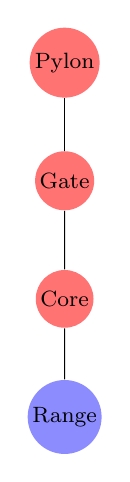
\begin{tikzpicture}
  [level distance=15mm,
   every node/.style={fill=red!55,circle,inner sep=1pt},
   level 1/.style={sibling distance=40mm},
   level 2/.style={sibling distance=20mm},
   level 3/.style={sibling distance=12mm}]
   \node {\begin{footnotesize}Pylon\end{footnotesize}}
   child {node {\begin{footnotesize}Gate\end{footnotesize}}
       child {node {\begin{footnotesize}Core\end{footnotesize}}
           %child {node {S}}
           %child [missing]
           %child {node {A}}
           child[techno] {node {\begin{footnotesize}Range\end{footnotesize}}}
       }
%    }
%child {node {F}
%    child {node {C}}
   };
\end{tikzpicture}
}
\hspace{2cm}
\ifthenelse{\equal{\myebookformat}{true}}{                   %%%%%%%%%%%%%%%%%%%%%%%%%%%
\includegraphics[width=5cm]{images/tikz9.png}  %%%%%%%%%%%%%%%%%%%%%%%%%%%
}{
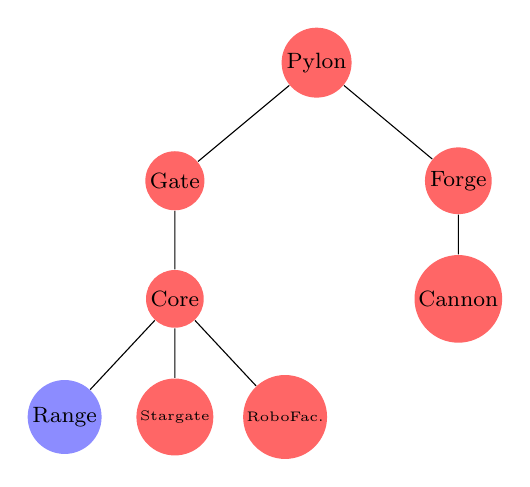
\begin{tikzpicture}
  [level distance=15mm,
   every node/.style={fill=red!60,circle,inner sep=1pt},
   level 1/.style={sibling distance=36mm},
   level 2/.style={sibling distance=20mm},
   level 3/.style={sibling distance=14mm}]
   \node {\begin{footnotesize}Pylon\end{footnotesize}}
   child {node {\begin{footnotesize}Gate\end{footnotesize}}
       child {node {\begin{footnotesize}Core\end{footnotesize}}
           child[techno] {node {\begin{footnotesize}Range\end{footnotesize}}}
           child {node {\begin{tiny}Stargate\end{tiny}}}
           child {node {\begin{tiny}RoboFac.\end{tiny}}}
       }
   }
child {node {\begin{footnotesize}Forge\end{footnotesize}}
    child {node {\begin{footnotesize}Cannon\end{footnotesize}}}
       };
\end{tikzpicture}
}
\end{center}
\caption{Two tech trees, the build trees subsets are the parts in red. Left: \glos{techtree} obtained at the end of the build order described in \ref{bo:two_gates_goon_range}. Right: a more advanced tech tree.}
\label{fig:buildtreetwogatesgoon}
\label{fig:techtreetwogatesgoonrange}
\end{figure}

\subsection{Attack Types}
With the discretization of the map into regions and choke-dependent regions, one can reason about \textit{where} attacks will happen. The types of the attacks depends on the units types involved and their use. There may be numerous variations but we decided to keep the four main types of attacks in the vocabulary of gamers:
\begin{itemize}
    \item \textit{ground} attacks, which may use all types of units (and so form the large majority of attacks). They are constrained by the map topography and by units collisions so chokes are very important: they are an advantage for the army with less contact units but enough ranged units or simply more ranged units, and/or the higher ground. 
    \item \textit{air} raids, air attacks, which can use only flying units. They are not constrained by the map, and the mobility of most flying units (except the largest) allows the player to attack quickly anywhere. Flying units are most often not cost-effective against ranged ground units, so their first role is to harass the economy (workers, tech buildings) and fight when in large numerical superiority (interception, small groups) or against units which cannot attack air units, all thanks to their mobility and ease of repositioning.
    \item \textit{invisible} (ground) attacks, which can use only a few specific units in each race (Protoss Dark Templars, Terran Ghosts, Zerg Lurkers). When detected, this units are not cost-effective. There are two ways to use invisible attacks: as an \textit{all-in} as soon as possible (because reaching the technology required to produce such units is costly and long), before that the enemy has detection technology. This is a risky strategy but with a huge payoff (sometimes simply the quick win of the game). The second way is to try and sneak invisible units behind enemy lines to sap the opponent's economy.
    \item \textit{drop} attacks, which need a transport unit (Protoss Shuttle, Terran Dropship, Zerg Overlord with upgrade). Transports give the mobility of flying units to ground units, with the downsides that units cannot fire when inside the transport. The usefulness of such attacks comes from the fact that they are immediately available as soon as the first transport unit is produced (because the ground units can be produced before it) and that they do not sacrifice cost-efficiency of most of the army. The downside is that transports are unarmed and are at the mercy of interceptions. The goals of such attacks are either to sap the opponent's economy (predominantly) or to quickly reinforce an army while maximizing micro-management of units.
\end{itemize}
The corresponding goal (orders) are described in section~\ref{sec:goals}.


\section{Dataset}
\label{sec:dataset}
\subsection{Source}
\newglossaryentry{metagame}{name={meta-game},description={preparation and maneuvering before (and between) games to exploit: current trends, opponent's style and weaknesses, map's specificities (safe zones, back doors, timings), and psychological ``mind games''.}}
% PvP 1336, PvT 7225, PvZ 6082, TvT 1384, TvZ 6322, ZvZ 598
We downloaded more than 8000 replays to keep 7649 uncorrupted, 1v1 replays from professional gamers leagues and international tournaments of StarCraft, from specialized websites\footnote{\url{http://www.teamliquid.net}}\footnote{\url{http://www.gosugamers.net}}\footnote{\url{http://www.iccup.com}}. We then ran them using BWAPI\footnote{\url{http://code.google.com/p/bwapi/}} and dumped units' positions, pathfinding and regions, resources, orders, vision events, for attacks: types, positions, outcomes. Basically, every BWAPI event plus attacks was recorded, the dataset and its source code are freely available\footnote{\url{http://snippyhollow.github.com/bwrepdump/}}. 
The implication of considering only replays of very good player allows us to use this dataset to learn the behaviors of our bot. Otherwise, particularly regarding the economy, a simple bot (AI) coupled with a planner can beat the average player, who does not have a tightly timed build order and/or not the sufficient \glos{APM} to execute. %carry it through. 
%The only downside of using human-played games of StarCraft to train our bot is that the \glos{metagame}, the strategic and psychological game in-between rounds that is, is very different for bots (inexistant) than for humans.


\subsection{Information}
Table~\ref{tab:dataset} shows some metrics about the dataset. In this chapter, we are particularly interested in the number of attacks. Note that there the numbers of attacks for a given race have to be divided by two in a given \textit{non-mirror} match-up. So, there are 7072 Protoss attacks in PvP but there are no 70,089 attacks by Protoss in PvT but about half that.
\begin{table}[h]
\begin{tabular}{|l|c|c|c|c|c|c|}
\hline
match-up & PvP & PvT & PvZ & TvT & TvZ & ZvZ \\
\hline
%%%number of games & 448 & 2412 & 2034 & 463 & 2108 & 200 \\ % with corrupted, numbers or .rep
number of games & 445 & 2408 & 2027 & 461 & 2107 & 199 \\
number of attacks & 7072 & 70089 & 40121 & 16446 & 42175 & 2162 \\
mean attacks/game & 15.89 & 29.11 & 19.79 & 35.67 & 20.02 & 10.86 \\
mean time (frames) / game & 32342 & 37772 & 39137 & 37717 & 35740 & 23898 \\
mean time (minutes) / game & 22.46 & 26.23 & 27.18 & 26.19 & 24.82 & 16.60 \\
mean regions / game & 19.59 & 19.88 & 19.69 & 19.83 & 20.21 & 19.31 \\
mean CDR / game & 41.58 & 41.61 & 41.57 & 41.44 & 42.10 & 40.70 \\
%actions issued (game engine) & 10939983 & 79968161 & 63535130 & 12446386 & 62935651 & 4351740 \\
actions issued (game engine) / game & 24584 & 33209 & 31344 & 26998 & 29869 & 21868 \\
mean ``BWAPI \glos{APM}''\footnote{the difference with the, real world, gamers' APM is that when the player issues an order to a group of $n$ units, it counts $n$ orders and thus $n$ actions (while it took one selection and one order, so 2 actions). Professional gamers' APM averages are about 300 with spikes above 500, and sustained rates of 400 during fights.} (per player) & 547 & 633 & 577 & 515 & 602 & 659 \\
mean ground distance\footnote{for regions connected by ground, pathfinding aware, in pixels} region $\leftrightarrow$ region & 2569 & 2608 & 2607 & 2629 & 2604 & 2596 \\ % divise by 32 for build tiles
mean ground distance\footnote{for choke-dependent regions connected by ground, pathfinding aware, in pixels} CDR $\leftrightarrow$ CDR & 2397 & 2405 & 2411 & 2443 & 2396 & 2401 \\ % divise by 32 for build tiles
\hline
\end{tabular}
\caption{Detailed numbers about our dataset. XvY means race X vs race Y matchs and is an abbreviation of the match-up: PvP stands for Protoss versus Protoss.}
\label{tab:dataset}
\end{table}

By running the recorded games (\gloss{replay}) through StarCraft, we were able to recreate the full state of the game. Time is always expressed in games frames (24 frames per second). We recorded three types of files:
\begin{itemize}
    \item general data (see appendix~\ref{fig:rgdfile}): records the players' names, the map's name, and all information about events like \textit{creation} (along with \textit{morph}), \textit{destruction}, \textit{discovery} (for one player), \textit{change of ownership} (special spell/ability), for each units. It also shows attack events (detected by a heuristic, see below) and dumps the current economical situation every 25 frames: \gloss{mineral}, \glos{gas}, \glos{supply} (count and total: \glos{maxsupply}).
    \item order data (see appendix~\ref{fig:rodfile}): records all the orders which are given to the units (individually) like \textit{move}, \textit{harvest}, \textit{attack unit}, the orders positions and their issue time.
    \item location data (see appendix~\ref{fig:rldfile}): records positions of mobile units every 100 frames, and their position in regions and choke-dependent regions if they changed since last measurement. It also stores ground distances (pathfinding-wise) matrices between regions and choke-dependent regions in the header.
\end{itemize}
From this data, one can recreate most of the state of the game: the map key characteristics (or load the map separately), the economy of all players, their \textit{tech} (all researches and upgrades), all the buildings and units, along with their orders and their positions.

\subsection{Attacks}
We trigger an attack tracking heuristic when one unit dies and there are at least two military units around. We then update this attack until it ends, recording every unit which took part in the fight. We log the position, participating units and fallen units for each player, the attack type and of course the attacker and the defender. Algorithm~\ref{alg:attackheuristic}\footnote{adapted from \url{http://github.com/SnippyHolloW/bwrepdump/blob/master/BWRepDump.cpp\#L1773} and \url{http://github.com/SnippyHolloW/bwrepdump/blob/master/BWRepDump.cpp\#L1147}} shows how we detect attacks.
\begin{algorithm}
\caption{Simplified attack tracking heuristic for extraction from games. The heuristics to determine the attack type and the attack radius and position are not described here. They look at the proportions of units types, which units are firing and the last actions of the players.}
%, adapted from \url{http://github.com/SnippyHolloW/bwrepdump/}} 
\label{alg:attackheuristic}
\begin{algorithmic}
\State $list tracked\_attacks$
\Function{unit\_death\_event}{$unit$}
    \State $tmp \leftarrow tracked\_attacks.which\_contains(unit)$
    \If{$tmp \neq \emptyset$}
        \State $tmp.update(unit)$ \Comment{$\Leftrightarrow update(tmp, unit)$}
    \Else
        \State $tracked\_attacks.push(attack(unit))$
    \EndIf
\EndFunction

\Function{attack}{$unit$} \Comment{new attack constructor}
    \State $self.convex\_enveloppe = propagate\_default\_enveloppe(unit)$ \Comment{$self \Leftrightarrow this$}
    \State $self.type \leftarrow determine\_attack\_type(update(self, unit))$
    \State \Return $self$
\EndFunction

\Function{update}{$attack, unit$}
    \State $attack.update\_enveloppe(unit)$ \Comment{takes units ranges into account}
    \State $c \leftarrow get\_context(attack.convex\_enveloppe)$
    \State $self.units\_involved.update(c)$ 
    \State $self.tick = default\_timeout()$
    \State \Return $c$
\EndFunction

\Function{tick\_update}{}
    \State $self.tick \leftarrow self.tick - 1$
    \If{$self.tick < 0$}
        \State $self.destruct()$
    \EndIf
\EndFunction
\end{algorithmic}
\end{algorithm}


\section{A Bayesian Tactical Model}
\label{sec:tacticalmodel}

\subsection{Tactical Model}

We preferred to map the continuous values from heuristics to a few discrete values to enable quick complete computations. Another strategy would keep more values and use Monte-Carlo sampling for computation. We think that discretization is not a concern because 1) heuristics are simple and biased already 2) we often reason about imperfect information and this uncertainty tops discretization fittings.

\subsubsection{Variables}
With $n$ regions, we have: 
\begin{itemize}
    \item $A_{1:n} \in \{true,false\}$, $A_i$: attack in region $i$ or not?
    \item $E_{1:n} \in \{no, low, high\}$, $E_i$ is the discretized economical value of the region $i$ for the defender. We choose 3 values: \textit{no} workers in the regions, \textit{low}: a small amount of workers (less than half the total) and \textit{high}: more than half the total of workers in this region $i$.
    \item $T_{1:n} \in discrete\ levels$, $T_i$ is the tactical value of the region $i$ for the defender, see above for an explanation of the heuristic. Basically, $T$ is proportional to the proximity to the defender's army. In benchmarks, discretization steps are $0,0.05,0.1,0.2,0.4,0.8$ ($log_2$ scale).
    \item $TA_{1:n} \in discrete\ levels$, $TA_i$ is the tactical value of the region $i$ for the attacker (as above but for the attacker instead of the defender).
    \item $B_{1:n} \in \{true, false\}$, $B_i$ tells if the region belongs (or not) to the defender. $\PP(B_i=true)=1$ if the defender has a base in region $i$ and $\PP(B_i=false)=1$ if the attacker has one. Influence zones of the defender can be measured (with uncertainty) by $\PP(B_i=true) \geq 0.5$ and vice versa.
    \item $H_{1:n} \in \{ground, air, invisible, drop\}$, $H_i$: in predictive mode: how we will be attacked, in decision-making: how to attack, in region $i$.
    \item $GD_{1:n} \in \{no, low, med, high\}$: ground defense (relative to the attacker power) in region $i$, result from a heuristic. \textit{no} defense if the defender's army is $\geq 1/10th$ of the attacker's, \textit{low} defense above that and under half the attacker's army, \textit{medium} defense above that and under comparable sizes, \textit{high} if the defender's army is bigger than the attacker.
    \item $AD_{1:n} \in \{no, low, med, high\}$: same for air defense.
    \item $ID_{1:n} \in \{no\ detector, one\ detector, several\}$: invisible defense, equating to numbers of detectors.
    \item $TT \in [\emptyset, building_1, building_2, building_1\wedge building_2, techtrees, \dots]$: all the possible technological trees for the given race. For instance $\{pylon, gate\}$ and $\{pylon, gate, core\}$ are two different $T$ech $T$rees, see chapter~\ref{chapter:strategy}.
    \item $HP \in \begin{small}\{ground, ground\wedge air, ground\wedge invis, ground\wedge air\wedge invis, ground\wedge drop, ground\wedge air\wedge drop, ground\wedge invis\wedge drop, ground\wedge air\wedge invis\wedge drop\}\end{small}$: \textbf{h}ow \textbf{p}ossible types of attacks, directly mapped from $TT$ information. This variable serves the purpose of extracting all that we need to know from $TT$ and thus reducing the complexity of a part of the model from $n$ mappings from $TT$ to $H_i$ to one mapping from $TT$ to $HP$ and $n$ mapping from $HP$ to $H_i$. Without this variable, learning the co-occurrences of $TT$ and $H_i$ is sparse in the dataset. In prediction, with this variable, we make use of what we can infer on the opponent's strategy \cite{SYNNAEVE:OpeningPred,SYNNAEVE:StratPred}, in decision-making, we know our own possibilities (we know our tech tree as well as the units we own).
    %\item
\end{itemize}
We can consider a more complex version of this tactical model taking soft evidences into account (variables on which we have a probability distribution), which is presented in appendix~\ref{appdx:softevidences}.

\subsubsection{Decomposition}
\label{sec:tacticaldecomposition}
\begin{eqnarray}
    & & \PP(A_{1:n}, E_{1:n}, T_{1:n}, TA_{1:n}, B_{1:n}, \\
& & H_{1:n}, GD_{1:n}, AD_{1:n}, ID_{1:n}, HP, TT) \\
    & = & \prod_{i=1}^n \left[\PP(A_i)\PP(E_i,T_i,TA_i,B_i|A_i) \label{eqn:tacticsdecomposition}\right.\\
& & \left. \PP(AD_i,GD_i,ID_i|H_i)\PP(H_i|HP)\right]\PP(HP|TT)\PP(TT)
\end{eqnarray}
This decomposition is also shown in Figure~\ref{fig:SpecialTacticsSimple_plate}. We can see that we have in fact two models: one for $A_{1:n}$ and one for $H_{1:n}$.

\begin{figure}[h]
\begin{center}
\includegraphics[width=9cm]{images/SpecialTacticsSimple_plate.pdf}
\caption{Plate diagram (factor graph notation) of the Bayesian tactical model.}
\label{fig:SpecialTacticsSimple_plate}
\end{center}
\end{figure}

\subsubsection{Forms and Learning}
\label{sec:tacticalidentification}
We will explain the forms for a given/fixed $i$ region number:
\begin{itemize}
\item $\PP(A)$ is the prior on the fact that the player attacks in this region, in our evaluation we set it to $n_{battles}/(n_{battles}+n_{not\ battles})$. 
\item $\PP(E,T,TA,B|A)$ is a co-occurrences table of the economical, tactical (both for the defender and the attacker), belonging scores where an attacks happen. We just use Laplace's law of succession (``add one'' smoothing) \cite{Jaynes} and count the co-occurrences in the games of the dataset (see~\ref{sec:dataset}), thus almost performing maximum likelihood learning of the table. 
\begin{small}
$$\PP(E=e,T=t,TA=ta,B=b|A=True) = \frac{1+n_{battles}(e,t,ta,b)}{\abs{E} \abs{T} \abs{TA} \abs{B} + \sum_{E,T,TA,B} n_{battles}(E,T,TA,B)}$$
\end{small}

%%% \item $\PP(\lambda_{B}|B,B') = 1.0\ iff\ B=B'$ is just a coherence constraint.

\item $\PP(AD,GD,ID|H)$ is a co-occurrences table of the air, ground, invisible defense values depending on how the attack happens. As for $\PP(E,T,TA,B|A)$, we use a Laplace's rule of succession learned from the dataset.
\begin{small}
$$\PP(AD=ad,GD=gd,ID=id|H=h) = \frac{1+n_{battles}(ad,gd,id,h)}{\abs{AD} \abs{GD} \abs{ID} + \sum_{AD,GD,ID} n_{battles}(AD,GD,ID,h)}$$
\end{small}

\item $\PP(H|HP)$ is the categorical distribution (histogram) on how the attack happens depending on what is possible. Trivially $\PP(H=ground|HP=ground)=1.0$, for more complex possibilities we have different smoothed maximum likelihood multinomial distributions on $H$ values depending on $HP$.
$$\PP(H=h|HP=hp) = \frac{1 + n_{battles}(h,hp)}{\abs{H} + \sum_{H} n_{battles}(H,hp)}$$

\item $\PP(HP|TT=tt)$ is a Dirac distribution on the $HP=hp$ which is compatible with $TT=tt$. It is the direct mapping of what the tech tree allows as possible attack types: $\PP(HP=hp|TT)=1$ is a function of $TT$ (all $\PP(HP\neq hp|TT)=0$).

\item $\PP(TT)$: if we are sure of the tech tree (prediction without fog of war, or in decision-making mode), $\PP(TT=k)=1$ and $\PP(TT\neq k)=0$; otherwise, it allows us to take uncertainty about the opponent's tech tree and balance $\PP(HP|TT)$. We obtain a distribution on what is possible ($\PP(HP)$) for the opponent's attack types.
\end{itemize}

There are two approaches to fill up these probability tables, either by observing games (supervised learning), as we did in the evaluation section, or by acting (reinforcement learning). %We first learned all the parameters from observations on the dataset. 

The model is highly modular, and some parts are more important than others. We can separate three main parts: $\PP(E,T,TA,B|A)$, $\PP(AD,GD,ID|H)$ and $\PP(H|HP)$. In prediction, $\PP(E,T,TA,B|A)$ uses the inferred (uncertain) economic ($E$), tactical ($T$) and belonging ($B$) scores of the opponent while knowing our own tactical position fully ($TA$). In decision-making, we know $E,T,B$ (for us) and estimate $TA$. In our prediction benchmarks, $\PP(AD,GD,ID|H)$ has the lesser impact on the results of the three main parts, either because the uncertainty from the attacker on $AD,GD,ID$ is too high or because our heuristics are too simple, though it still contributes positively to the score. In decision-making, it allows for reinforcement learning to have pivoting tuple values for $AD,GD,ID$ at which to switch attack types. In prediction, $\PP(H|HP)$ is used to take $\PP(TT)$ (coming from strategy prediction \citep{SYNNAEVE:StratPred}, chapter~\ref{chapter:strategy}) into account and constraints $H$ to what is possible. For the use of $\PP(H|HP)\PP(HP|TT)\PP(TT)$ in decision-making, see the \textit{results} section (\ref{sec:tacticalresults}) or the appendix~\ref{appdx:softevidences}.

\subsubsection{Questions}
For a given region $i$, we can ask the probability to attack here,
%%% \begin{equation}
%%% \PP(A_i=a_i|e_i,t_i,ta_i,\lambda_{B,i}=1)
%%% \end{equation}
%%% \begin{small}
%%% \begin{equation}
%%% = \frac{\sum_{B_i,B_i'}\PP(e_i,t_i,ta_i,B_i|a_i)\PP(a_i)\PP(B_i').P(\lambda_{B,i}|B_i,B_i')}{\sum_{A_i,B_i,B_i'}\PP(e_i,t_i,ta_i,B_i|A_i)\PP(A_i)\PP(B_i')\PP(\lambda_{B,i}|B_i,B_i')}
%%% \end{equation}
%%% \end{small}
%%% \begin{equation}
%%% \propto \sum_{B_i,B_i'}\PP(e_i,t_i,ta_i,B_i|a_i)\PP(a_i)\PP(B_i')\PP(\lambda_{B,i}|B_i,B_i')
%%% \end{equation}
\begin{eqnarray}
& & \PP(A_i=a_i|e_i,t_i,ta_i,b_i)\\
& = &\frac{\PP(e_i,t_i,ta_i,b_i|a_i)\PP(a_i)}{\sum_{A_i}\PP(e_i,t_i,ta_i,b_i|A_i)\PP(A_i)}\\
& \propto & \PP(e_i,t_i,ta_i,B_i|a_i)\PP(a_i)
\end{eqnarray}
and the mean by which we should attack,
\begin{eqnarray}
& & \PP(H_i=h_i|ad_i,gd_i,id_i) \\
& \propto & \sum_{TT,HP}[\PP(ad_i,gd_i,id_i|h_i)\PP(h_i|HP)\PP(HP|TT)\PP(TT)]
\end{eqnarray}
%For clarity, we omitted some variables couples on which we have to sum (to take uncertainty into account) as for $B$ (and $B'$) above. 
We always sum over estimated, inferred variables, while we know the one we observe fully. In prediction mode, we sum over $TA,B,TT,HP$; in decision-making, we sum over $E,T,B,AD,GD,ID$ (see appendix~\ref{appdx:softevidences}). 
The complete question that we ask our model is $\PP(A,H|FullyObserved)$. The maximum of $\PP(A,H)=\PP(A)\times \PP(H)$ may not be the same as the maximum of $\PP(A)$ or $\PP(H)$ take separately. For instance think of a very important economic zone that is very well defended, it may be the maximum of $\PP(A)$, but not once we take $\PP(H)$ into account. Inversely, some regions are not defended against anything at all but present little or no interest. Our joint distribution \ref{eqn:tacticsdecomposition} can be rewritten: $\PP(Searched,FullyObserved,Estimated)$, so we ask:
\begin{eqnarray}
& & \PP(A_{1:n},H_{1:n}|FullyObserved) \label{eqn:tacticsquestion}\\
& \propto & \sum_{Estimated}\PP(A_{1:n},H_{1:n},Estimated,FullyObserved)
\end{eqnarray}

The Bayesian program of the model is as follows:% (\ref{bp:BayesianTactician}):
\begin{eqnarray*}
\begin{sideways}\parbox{35mm}{\hspace{-1.3cm}Bayesian program}\end{sideways}
\begin{cases}
\begin{sideways}\parbox{15mm}{\hspace{-0.8cm}Description}\end{sideways}
    \begin{cases}
    
\begin{sideways}\parbox{35mm}{\hspace{-1.1cm}Specification ($\pi$)}\end{sideways}
        \begin{cases}
        Variables\\
A_{1:n}, E_{1:n}, T_{1:n}, TA_{1:n}, B_{1:n}, B'_{1:n}, \lambda_{B,1:n},\\
H_{1:n}, GD_{1:n}, AD_{1:n}, ID_{1:n}, HP, TT\\
        Decomposition\\
\PP(A_{1:n}, E_{1:n}, T_{1:n}, TA_{1:n}, B_{1:n}, B'_{1:n}, \lambda_{B,1:n}, \\
H_{1:n}, GD_{1:n}, AD_{1:n}, ID_{1:n}, HP, TT) \\
= \prod_{i=1}^n \left[\PP(A_i)\PP(E_i,T_i,TA_i,B_i|A_i)\right.\\
\PP(\lambda_{B,i} | B_{1:n},B'_{1:n})\PP(B'_{1:n}) \\
\left. \PP(AD_i,GD_i,ID_i|H_i)\PP(H_i|HP)\right]\PP(HP|TT)\PP(TT)\\
        Forms\\
\PP(A)\ \mathrm{prior\ on\ attack\ in\ region}\ i\\
\PP(E,T,TA,B|A)\ \mathrm{covariance/probability\ table}\\ 
\PP(\lambda_{B}|B,B') = 1.0\ iff\ B=B',\ else\ \PP(\lambda_{B}|B,B') = 0.0\ (functional\ Dirac)\\ 
\PP(AD,GD,ID|H)\ \mathrm{covariance/probability\ table}\\
\PP(H|HP) = Categorical(4,HP)\\
\PP(HP=hp|TT) = 1.0\ iff\ TT\rightarrow hp,\ else\ \PP(HP|TT)=0.0\\
\PP(TT)\ \mathrm{comes\ from\ a\ strategic\ model}\\
        \end{cases}\\
    Identification\ (using\ \delta)\\
\PP(A=true)= \frac{n_{battles}}{n_{battles}+n_{not\ battles}} = \frac{\mu_{battles/game}}{\mu_{regions/map}}\ \mathrm{(probability\ to\ attack\ a\ region)}\\
\mathrm{it\ could\ be\ learned\ online\ (preference\ of\ the\ opponent):}\\
\PP(A_r=true) = \frac{1 + n_{battles}(r)}{2 + \sum_{i \in regions}n_{battles}(i)}\ \mathrm{(online\ for\ each\ game\ }\forall r\mathrm{)}\\
\PP(E=e,T=t,TA=ta,B=b|A=True) = \frac{1+n_{battles}(e,t,ta,b)}{\abs{E} \times \abs{T} \times \abs{TA} \times \abs{B} + \sum_{E,T,TA,B} n_{battles}(E,T,TA,B)} \\
\PP(AD=ad,GD=gd,ID=id|H=h) = \frac{1+n_{battles}(ad,gd,id,h)}{\abs{AD} \times \abs{GD} \times \abs{ID} + \sum_{AD,GD,ID} n_{battles}(AD,GD,ID,h)} \\
\PP(H=h|HP=hp) = \frac{1 + n_{battles}(h,hp)}{\abs{H} + \sum_{H} n_{battles}(H,hp)}\\
    \end{cases}\\
Questions\\
\forall i \in regions \PP(A_i|e_i,t_i,ta_i,\lambda_{B,i}=1)\\
\forall i \in regions \PP(H_i|ad_i,gd_i,id_i) \\
\PP(A,H|FullyObserved)\\
\end{cases}
\label{bp:BayesianTactician}
\end{eqnarray*}


\section{Results on StarCraft}
\label{sec:tacticalresults}

\subsection{Learning}
To measure fairly the prediction performance of such a model, we applied ``leave-100-out'' cross-validation from our dataset: as we had many games (see Table.~\ref{tab:all_results}), we set aside 100 games of each match-up for testing (with more than 1 battle per match: rather $\approx 15$ battles/match) and train our model on the rest. We write match-ups XvY with X and Y the first letters of the factions involved (Protoss, Terran, Zerg). Note that mirror match-ups (PvP, TvT, ZvZ) have fewer games but twice as many attacks from a given faction. Learning was performed as explained in III.B.3: for each battle in $r$ we had one observation for: $\PP(e_r,t_r,ta_r,b_r|A=true)$, and $\#regions-1$ observations for the $i$ regions which were not attacked: $\PP(e_{i \neq r},t_{i \neq r}, ta_{i \neq r}, b_{i \neq r}|A=false)$. For each battle of type $t$ we had one observation for $P(ad,gd,id|H=t)$ and $P(H=t|p)$. By learning with a Laplace's law of succession \cite{Jaynes}, we allow for unseen event to have a non-zero probability.

An exhaustive presentation of the learned tables is out of the scope of this chapter, but we displayed interesting cases in which the learned probability tables meet concur with human expertise in Figures~\ref{fig:P_H_AD},~\ref{fig:PossibleP} and \ref{fig:Where3D}. In Fig.~\ref{fig:P_H_AD}, we see that air raids/attacks are quite risk averse and it is two times more likely to attack a region with less than 1/10th of the flying force in anti-aircraft warfare than to attack a region with up to one half of our force. We can also notice than drops are to be preferred either when it is safe to land (no anti-aircraft defense) or when there is a large defense (harassment tactics). In Fig.~\ref{fig:PossibleP} we can see that, in general, there are as many ground attacks at the sum of other types. The two top graphs show cases in which the tech of the attacker was very specialized, and, in such cases, the specificity seems to be used. In particular, the top right graphic may be corresponding to a ``fast Dark Templars rush''. Finally, Fig.~\ref{fig:Where3D} shows the transition between two types of encounters: tactics aimed at engaging the enemy army (a higher $T$ value entails a higher $\PP(A)$) and tactics aimed at damaging the enemy economy (at high $E$, we look for opportunities to attack with a small army where $T$ is lower).

\begin{figure}[!h]
\centerline{\includegraphics[width=11cm]{images/Terran_Prob_H_crop.png}}
%\caption{$\PP(H=air)$ and $\PP(H=drop)$ for varying values of $AD$ (summed on other variables), for Terran in TvP.}
\caption{(top) $\PP(H=invis)$ and $\PP(H=drop)$ for varying values of $GD$ (summed on other variables); (bottom) $\PP(H=air)$ and $\PP(H=drop)$ for varying values of $AD$ (summed on other variables), for Terran in TvP. We can see that it is far more likely that invisible (``sneaky'') attacks happen where there is low ground presence (top left plot). For drops, we understand that the high value for $\PP(H=drop|GD=1.0)$ is caused by the fact that drop armies are small and this value corresponds to drops which are being expected by the defender. Drops at lower values of $GD$ correspond to unexpected (surprise) drops. As ground units are more cost efficient than flying units in a static battle, we see that both $\PP(H=invis|AD=0.0)$ and $\PP(H=drop|AD=0.0)$ are much more probable than situations with air defenses.}
\label{fig:P_H_AD}
%\vspace{-0.5cm}
\end{figure}

\begin{figure}[!h]
\centerline{\includegraphics[width=11cm]{images/PossibleP.png}}
%\caption{$\PP(H|HP)$ for varying values $H$ and for different values of $P$ (derived from inferred $TT$), for Protoss in PvT.}
\caption{$\PP(H|HP)$ for varying values of $H$ and for different values of $P$ (derived from inferred $TT$), for Protoss in PvT. Conditioning on what is possible given the \textit{tech tree} gives a lot of information about what attack types are possible or not. More interestingly, it clusters the game phases in different tech levels and allows for learning the relative distributions of attack types with regard to each phase. For instance, the last (bottom right) plot shows the distribution on attack types at the end of a technologically complete game.}
\label{fig:PossibleP}
\end{figure}

\begin{figure}[!h]
\centerline{\includegraphics[width=9cm]{images/where3D_EI_TI_RegT.png}}
%\caption{$\PP(A)$ for varying values of $E$ and $T$, summed on the other variables, for Terran in TvT.}
\caption{$\PP(A)$ for varying values of $E$ and $T$, summed on the other variables, for Terran in TvT. Higher economical values is strongly correlated with surprise attacks with small tactical squads and no defenses, which almost never happens in open fields (``no eco'') as this would lead to very unbalanced battles (in terms of army sizes): it would not benefit the smaller party, which can flee and avoid confrontation, as opposed to when defending their base.}
\label{fig:Where3D}
%\vspace{-0.5cm}
\end{figure}

\subsection{Prediction Performance}
We learned and tested one model for each race and each match-up. As we want to predict \textit{where} ($\PP(A_{1:n})$) and \textit{how} ($\PP(H_{battle})$) the next attack will happen to us, we used inferred enemy $TT$ (to produce $P$) and $TA$, our scores being fully known: $E$, $T$, $B$, $ID$. We consider $GD$, $AD$ to be fully known even though they depend on the attacker force, we should have some uncertainty on them, but we tested that they accounted (being known instead of fully unknown) for 1 to 2\% of $\PP(H)$ accuracy (in prediction) once $P$ was known. We should point that pro-gamers scout very well and so it allows for a highly accurate $TT$ estimation with \cite{SYNNAEVE:StratPred}. Training requires to recreate battle states (all units' positions) and count parameters for 5,000 to 30,000 battles. Once that is done, inference is very quick: a look-up in a probability table for known values and $\#F$ look-ups for free variables $F$ on which we sum. We chose to try and predict the next battle 30 seconds before it happens, 30 seconds being an approximation of the time needed to go from the middle of a map (where the entropy on ``next battle position'' is maximum as the army's average distance to all other regions is minimal) to any region by ground, so that the prediction is useful for the defender (they can position their army).

The model code\footnote{\url{https://github.com/SnippyHolloW/AnalyzeBWData}} (for learning and testing) as well as the datasets (see above) are freely available. Raw results of predictions of positions and types of attacks 30 seconds before they happen are presented in Table.~\ref{tab:all_results}: for instance the bold number (38.0) corresponds to the percentage of good positions (regions) predictions (30 sec before event) which were ranked 1st in the probabilities on $A_{1:n}$ for Protoss attacks against Terran (PvT). The measures on \textit{where} corresponds to the percentage of good prediction and the mean probability for given ranks in $\PP(A_{1:n})$ (to give a sense of the shape of the distribution). As the most probable The measures on \textit{how} corresponds to the percentage of good predictions for the most probable $\PP(H_{battle})$ and the number of such battles seen in the test set for given attack types. We particularly predict well ground attacks (trivial in the early game, less in the end game) and, interestingly, Terran and Zerg drop attacks. The \textit{where \& how} row corresponds to the percentage of good predictions for the maximal probability in the joint $\PP(A_{1:n},H_{1:n})$: considering only the most probable attack (more information is in the rest of the distribution, as shown for \textit{where}!) according to our model, we can predict \textit{where} \textbf{and} \textit{how} an attack will occur in the next 30 seconds $\approx$ 1/4th of the time. 

Finally, note that scores are still good 60 seconds before the attack (obviously, $TT$, and thus $P$, are not so different, nor are $B$ and $E$): PvT \textit{where} top 4 ranks are 35.6, 8.5, 7.7, 7.0\% good versus 38.0, 16.3, 8.9, 6.7\% 30 seconds before; \textit{how} total precision 60 seconds before is 70.0\% vs. 72.4\%, \textit{where \& how} maximum probability precision is 19.9\% vs. 23\%. This gives even more time for the player to adapt their tactics.

\setlength{\tabcolsep}{4.69pt}
\begin{sidewaystable}[!h]
\caption{Results summary for multiple metrics at 30 seconds before attack. The number in bold (38.0) is read as ``38\% of the time, the region $i$ with probability of rank 1 in $\PP(A_i)$ is the one in which the attack happened 30 seconds later''.}
\begin{center}
%\begin{small}
\begin{footnotesize}
\begin{tabular}{|cc|cc|cc|cc|cc|cc|cc|cc|cc|cc|}
\hline
\multicolumn{2}{|c|}{\%: good predictions} & \multicolumn{6}{||c|}{Protoss} & \multicolumn{6}{|c|}{Terran} & \multicolumn{6}{|c|}{Zerg} \\
\multicolumn{2}{|c|}{Pr: mean probability} & \multicolumn{2}{||c|}{P} & \multicolumn{2}{|c|}{T} & \multicolumn{2}{|c|}{Z} & \multicolumn{2}{|c|}{P} & \multicolumn{2}{|c|}{T} & \multicolumn{2}{|c|}{Z} & \multicolumn{2}{|c|}{P} & \multicolumn{2}{|c|}{T} & \multicolumn{2}{|c|}{Z} \\
\hline
% PvP 1336, PvT 7225, PvZ 6082, TvT 1384, TvZ 6322, ZvZ 598
\multicolumn{2}{|c|}{total \# games} & \multicolumn{2}{|c|}{1336} & \multicolumn{2}{|c|}{7225}& \multicolumn{2}{|c|}{6082}& \multicolumn{2}{|c|}{7225}& \multicolumn{2}{|c|}{1384}& \multicolumn{2}{|c|}{6322}& \multicolumn{2}{|c|}{6082}& \multicolumn{2}{|c|}{6322}& \multicolumn{2}{|c|}{598}\\
\hline
measure & rank & \% & Pr & \% & Pr & \% & Pr & \% & Pr & \% & Pr& \% & Pr& \% & Pr& \% & Pr& \% & Pr  \\
\hline
 & 1 & 40.9 & .334 & \textbf{38.0} & .329 & 34.5 & .304 & 35.3 & .299 & 34.4 & .295 & 39.0 & 0.358 & 32.8 & .31 & 39.8 & .331 & 37.2 & .324 \\
\multirow{3}{3mm}{\begin{sideways}\parbox{3mm}{\begin{small}where\end{small}}\end{sideways}}
 & 2 & 14.6 & .157 & 16.3 & .149 & 13.0 & .152 & 14.3 & .148 & 14.7 & .0147 & 17.8 & .174 & 15.4 & .166 & 16.6 & .148 & 16.9 & .157 \\
 & 3 & 7.8 & .089 & 8.9 & .085 & 6.9 & .092 & 9.8 & .09 & 8.4 & .087 & 10.0 & .096 & 11.3 & .099 & 7.6 & .084 & 10.7 & .100 \\
 & 4 & 7.6 & .062 & 6.7 & .059 & 7.9 & .064 & 8.6 & .071 & 6.9 & .063 & 7.0 & .062 & 8.9 & .07 & 7.7 & .064 & 8.6 & .07 \\
%\multicolumn{2}{|c|}{distance best} & \multicolumn{2}{|c|}{32} &\\
\hline
measure & type & \% & N & \% & N & \% & N & \% & N & \% & N & \% & N & \% & N & \% & N & \% & N \\
\hline
 & G & 97.5 & 1016 & 98.1 & 1458 & 98.4 & 568 & 100 & 691 & 99.9 & 3218 & 76.7 & 695 & 86.6 & 612 & 99.8 & 567 & 67.2 & 607 \\
\multirow{3}{3mm}{\begin{sideways}\parbox{3mm}{\begin{small}how\end{small}}\end{sideways}}
 & A & 44.4 & 81 & 34.5 & 415 & 46.8 & 190 & 40 & 5 & 13.3 & 444 & 47.1 & 402 & 14.2 & 155 & 15.8 & 19 & 74.2 & 586 \\
 & I & 22.7 & 225 & 49.6 & 337 & 12.9 & 132 & NA & NA & NA & NA & 36.8 & 326 & 32.6 & 227 & NA & NA & NA & NA \\
 & D & 55.9 & 340 & 42.2 & 464 & 45.2 & 93 & 93.5 & 107 & 86 & 1183 & 62.8 & 739 & 67.7 & 535 & 81.4 & 86 & 63.6 & 588 \\
\multicolumn{2}{|c|}{total} & 76.3 & 1662 & 72.4 & 2674 & 71.9 & 983 & 98.4 & 806 & 88.5 & 4850 & 60.4 & 2162 & 64.6 & 1529 & 94.7 & 674 & 67.6 & 1802 \\
\hline
\multicolumn{2}{|c|}{where \& how (\%)} & \multicolumn{2}{|c|}{32.8} & \multicolumn{2}{|c|}{23}& \multicolumn{2}{|c|}{23.8}& \multicolumn{2}{|c|}{27.1}& \multicolumn{2}{|c|}{23.6}& \multicolumn{2}{|c|}{30.2}& \multicolumn{2}{|c|}{23.3}& \multicolumn{2}{|c|}{30.9}& \multicolumn{2}{|c|}{26.4}\\
\hline
\end{tabular}
\label{tab:all_results}
\end{footnotesize}
%\end{small}
\end{center}
\end{sidewaystable}

When we are mistaken, the mean ground distance (pathfinding wise) of the most probable predicted region to the good one (where the attack happens) is 1223 pixels (38 build tiles, or 2 screens in StarCraft's resolution), while the mean max distance on the map is 5506 (172 build tiles). Also, the mean number of regions by map is 19, so a random \textit{where} (attack destination) picking policy would have a correctness of 1/19 (5.23\%). For choke-centered regions, the numbers of good \textit{where} predictions are lower (between 24\% and 32\% correct for the most probable) but the mean number of regions by map is 42. For \textit{where \& how}, a random policy would have a precision of 1/(19*4), and even a random policy taking the high frequency of ground attacks into account would at most be $\approx$ 1/(19*2) correct. 
%For the location only (\textit{where} question), we also considered a \textit{baseline} heuristic (learned from data) whic knows the most probable regions to be attacked (given the map and the start locations of both players, which makes the dataset quite sparse). This heuristic would give (depending on the match-up) prediction rates between 20.5 and 25.2\% for regions, and between 16.1\% and 19.5\% for choke-dependent regions. 
For the location only (\textit{where} question), we also counted the mean number of different regions which were attacked in a given game (between 3.97 and 4.86 for regions, depending on the match-up, and between 5.13 and 6.23 for choke-dependent regions). The ratio over these means would give the best prediction rate we could expect from a \textit{baseline heuristic} based solely on the location data. These are attacks that actually happened, so the number of regions a player have to be worried about is at least this one (or more, for regions which were not attacked during a game but were potential targets). This \textit{baseline heuristic} would yield (depending on the match-up) prediction rates between 20.5 and 25.2\% for regions, versus our 32.8 to 40.9\%, and between 16.1\% and 19.5\% for choke-dependent regions, versus our 24\% to 32\%.
%{'Reg': 3.9731182795698925, 'CDR': 5.123655913978495}
%{'Reg': 4.8563829787234045, 'CDR': 6.223404255319149}
Note that our current model consider a uniform prior on regions (no bias towards past battlefields) and that we do not incorporate any derivative of the armies' movements. There is no player modeling at all: learning and fitting the mean player's tactics is not optimal, so we should specialize the probability tables for each player. Also, we use all types of battles in our training and testing. Short experiments showed that if we used only attacks on bases, the probability of good \textit{where} predictions for the maximum of $\PP(A_{1:n})$ goes above 50\% (which is not a surprise, there are far less bases than regions in which attacks happen). To conclude on tactics positions prediction: if we sum the 2 most probable regions for the attack, we are right at least half the time; if we sum the 4 most probable (for our robotic player, it means it prepares against attacks in 4 regions as opposed to 19), we are right $\approx$ 70\% of the time.

Mistakes on the type of the attack are high for invisible attacks: while these tactics can definitely win a game, the counter is strategic (it is to have detectors technology deployed) more than positional. Also, if the maximum of $\PP(H_{battle})$ is wrong, it doesn't mean than $\PP(H_{battle}=good)=0.0$ at all! The result needing improvements the most is for air tactics, because countering them really is positional, see our discussion in the conclusion.
% distances
% mean: 1047 + 1134 + 1266 + 1257 + 1306 + XXX + 1228 + 1067 + 1480
% max: 5494 + 5605 + 5433 + 5558 + 5475 + 5443
% best CDR: 32%, 29%, 24%, 24%, 26%, XXX, 25%, 28%, 29%

\subsection{In Game Decision-Making}
In a StarCraft game, our bot has to make decisions about where and how to attack or defend, it does so by reasoning about opponent's tactics, bases, its priors, and under strategic constraints (Fig.~\ref{conceptTACTICS}). Once a decision is taken, the output of the tactical model is an offensive or defensive goal. There are different military goal types (base defense, ground attacks, air attacks, drops...), and each type of goal has pre-requisites (for instance: a drop goal needs to have the control of a dropship and military units to become active). The spawned goal then autonomously sets objectives for Bayesian units \cite{SYNNAEVE:Micro}, sometimes procedurally creating intermediate objectives or canceling itself in the worst cases. 

The destinations of goals are from $\PP(A)$, while the type of the goal comes from $\PP(H)$. In input, we fully know tactical scores of the regions according to our military units placement $TA$ (we are the attacker), what is possible for us to do $P$ (according to units available) and we estimate $E$, $T$, $B$, $ID$, $GD$, $AD$ from past (partial) observations. Estimating $T$ is the most tricky of all because it may be changing fast, for that we use a units filter which just decays probability mass of seen units. An improvement would be to use a particle filter \cite{weber2011aiide}, with a learned motion model. From the joint \ref{eqn:tacticsquestion} $\PP(A_{1:n},H_{1:n}|ta,p,tt)$ may arise a couple $i,H_i$ more probable than the most probables $\PP(A_i)$ and $\PP(H_j)$ taken separately (the case of an heavily defended main base and a small unprotected expand for instance). Fig.~\ref{fig:WhereHow} displays the mean $\PP(A,H)$ for Terran (in TvZ) attacks decision-making for the most 32 probable type/region tactical couples. It is in this kind of landscape (though more steep because Fig.~\ref{fig:WhereHow} is a mean) that we sample (or pick the most probable couple) to take a decision. Also, we may spawn defensive goals countering the attacks that we predict from the opponent.

\begin{figure}[!h]
\centerline{\includegraphics[width=9cm]{images/WhereHow_T_TvZ_light.png}}
%\vspace{-0.3cm}
% \caption{Mean $\PP(A,H)$ for all $H$ values and the top 8 $\PP(A_i,H_i)$ values, for Terran in TvZ. The larger the white square area, the higher $\PP(A_i,H_i)$.}
\caption{Mean $\PP(A,H)$ for all $H$ values and the top 8 $\PP(A_i,H_i)$ values, for Terran in TvZ. The larger the white square area, the higher $\PP(A_i,H_i)$. A simple way of taking a tactical decision according to this model, and the learned parameters, is by sampling in this distribution.}
\label{fig:WhereHow}
%\vspace{-0.5cm}
\end{figure}

Finally, we can steer our technological growth towards the opponent's weaknesses. A question that we can ask our model (at time $t$) is $\PP(TT)$, or, in two parts: we first find $i,h_i$ which maximize $\PP(A,H)$ at time $t+1$, and then ask a more directive:
$$\PP(TT|h_i) \propto \sum_{P} \PP(h_i|HP)\PP(HP|TT)\PP(TT)$$
so that it gives us a distribution on the tech trees ($TT$) needed to be able to perform the wanted attack type. To take a decision on our technology direction, we can consider the distances between our current $tt^t$ and all the probable values of $TT^{t+1}$.

\section{Discussion}
%\subsection{Possible Improvements}
There are three main research directions for possible improvements:
\begin{itemize}
    \item improving the underlying heuristics: the heuristics presented here are quite simple but they may be changed, and even removed or added, for another RTS or FPS, or for more performance. In particular, our ``defense against invisible'' heuristic could take detector positioning/coverage into account. Our heuristic on tactical values can also be reworked to take terrain tactical values into account (chokes and elevation in StarCraft). For the estimated position of enemy units, we could use a particle filter \cite{weber2011aiide} with a motion model (at least one for ground units and one for flying units). 
    \item improving the dynamic of the model: there is room to improve the dynamics of the model: considering the prior probabilities to attack in regions given past attacks and/or considering evolutions of the $T$,$TA$,$B$,$E$ values (derivatives) in time. The discretizations that we used may show their limits, though if we want to use continuous values, we need to setup a more complicated learning and inference process (MCMC sampling).
    \item improving the model itself: finally, one of the strongest assumptions (which is a drawback particularly for prediction) of our model is that the attacking player is always considered to attack in this most probable regions. While this would be true if the model was complete (with finer army positions inputs and a model of what the player thinks), we believe such an assumption of completeness is far fetched. Instead we should express that incompleteness in the model itself and have a ``player decision'' variable $D \sim Multinomial(\PP(A_{1:n},H_{1:n}),player)$.
\end{itemize} 

% TODO discuss, improvements, links
% TODO OR NOT Real-time A* (RTA) \citep{Korf88} can help in generating subgoals earning the heuristic by which // for automatic selection of subgoals in pathfinding, \citep{BulitkoBL10} case-based subgoaling

We have presented a Bayesian tactical model for RTS AI, which allows both for opposing tactics prediction and autonomous tactical decision-making. Being a probabilistic model, it deals with uncertainty easily, and its design allows easy integration into multi-granularity (multi-scale) AI systems as needed in RTS AI. Without any temporal dynamics, the position prediction is above a baseline heuristic ([32.8-40.9\%] vs [20.5-25.2\%]). Moreover, its exact prediction rate of the joint position and tactical type is in [23-32.8]\% (depending on the match-up), and considering the 4 most probable regions it goes up to $\approx$ 70\%. More importantly, it allows for tactical decision-making under (technological) constraints and (state) uncertainty. It can be used in production thanks to its low CPU and memory footprint. The dataset, its documentation\footnote{\url{http://snippyhollow.github.com/bwrepdump/}}, as well as our model implementation\footnote{\url{https://github.com/SnippyHolloW/AnalyzeBWData}} (and other data-exploration tools) are free software and can be found online. We plan to use this model in our StarCraft AI competition entry bot as it gives our bot tactical autonomy and a way to adapt to our opponent.

In a given match it should be initialized to uniform and progressively learn the preferred attack regions of the opponent for predictions, learn the regions in which our attacks fail or succeed for decision-making. % TODO
In match situation against a given opponent, for inputs that we can unequivocally attribute to their intention (style and general strategy), we also refine these probability tables (with Laplace's rule of succession). To keep things simple, we just refine $\sum_{E,T,TA}\PP(E,T,TA,B|A)$ corresponding to their aggressiveness (aggro) or our successes and failures, and equivalently for $\PP(H|HP)$. Indeed, if we sum over $E$, $T$ and $TA$, we consider the inclination of our opponent to venture into enemy territory or the interest that we have to do so by counting our successes with aggressive or defensive parameters. In $\PP(H|HP)$, we are learning the opponent's inclination for particular types of tactics according to what is available to their, or for us the effectiveness of our attack types choices. %TODO


The advantages are that 1) learning will adapt the model output to its biased heuristic inputs 2) the model is agnostic to where input variables' values come from 3) the updating process is the same for offline and online (in-game) learning. % TODO

Our approach (and bot architecture, depicted in Fig.~\ref{fig:conceptTACTICS}) can be seen as goal-driven autonomy \cite{Weber2010cr} dealing with multi-level reasoning by passing distributions (without any assumption about how they were obtained) on the module input. Using distributions as messages between specialized modules makes dealing with uncertainty first class, this way a given model do not care if the uncertainty comes from incompleteness in the data, a complex and biased heuristic, or another probabilistic model. We then take a decision by sampling or taking the most probable value in the output distribution. Another particularity of our model is that it allows for prediction of the enemy tactics using the same model with different inputs. Finally, our approach is not exclusive to most of the techniques presented above, and it could be interesting to combine it with UCT \citep{UCT} and more complex/precise tactics generated through planning \citep{Chung05} % TODO
